% \documentclass[11pt]{article}

% \usepackage[left=1in,right=1in,top=1in,bottom=1in]{geometry}

% \usepackage{graphics,epsfig,graphicx,float,subfigure,color}
% \usepackage{algorithm,algorithmic}
% \usepackage{amsmath,amssymb,amsbsy,amsfonts,amsthm}
% \usepackage[small,bf,up]{caption}

% \usepackage{soul}
% \usepackage{comment}
% \usepackage{url}
% \usepackage{boxedminipage}
% \usepackage[sf,bf,small]{titlesec}
% \usepackage[textsize=footnotesize]{todonotes}
% \usepackage[plainpages=false, colorlinks=true,
%    citecolor=blue, filecolor=blue, linkcolor=blue,
%    urlcolor=blue]{hyperref}

% \usepackage{amsmath}

% \include{ogmacros}

% \newcommand{\bdm}{\begin{displaymath}}
% \newcommand{\edm}{\end{displaymath}}

% \newcommand{\ben}{\begin{enumerate}}
% \newcommand{\een}{\end{enumerate}}

% \newcommand{\p}{\partial}
% \newcommand{\bs}{\boldsymbol}

% \usepackage{amssymb}
\documentclass[11pt]{article}

\usepackage[left=1in, right=1in, top=1in, bottom=1in, paperwidth=8.5in, paperheight=30in]{geometry} % Adjust 'paperheight' as needed

\usepackage{graphics,epsfig,graphicx,float,subfigure,color}
\usepackage{algorithm,algorithmic}
\usepackage{amsmath,amssymb,amsbsy,amsfonts,amsthm}
\usepackage[small,bf,up]{caption}


\usepackage{soul}
\usepackage{comment}
\usepackage{url}
\usepackage{boxedminipage}
\usepackage[sf,bf,small]{titlesec}
\usepackage[textsize=footnotesize]{todonotes}
\usepackage[plainpages=false, colorlinks=true,
   citecolor=blue, filecolor=blue, linkcolor=blue,
   urlcolor=blue]{hyperref}

\usepackage{amsmath}

\include{ogmacros}

\newcommand{\bdm}{\begin{displaymath}}
\newcommand{\edm}{\end{displaymath}}

\newcommand{\ben}{\begin{enumerate}}
\newcommand{\een}{\end{enumerate}}

\newcommand{\p}{\partial}
\newcommand{\bs}{\boldsymbol}

\usepackage{amssymb}

%$\mathbb{R}$

\parskip 1ex

\parindent 0ex

\begin{document}
\pagestyle{empty}

\begin{center}
{\large {\bf MATH 140: Mathematical Methods for Optimization}}\\
{\bf Assignment 5---Spring 2024}\\
{\bf Due February 22, 2024} \\
{\textcolor{red}{\bf By:Ronald Nap}}

\end{center}

\begin{enumerate}

  \item ({\bf 10 points}) Consider the unconstrained optimization
    problem (as in hw \#4)
    \bdm \min f(x,y) \equiv - \cos x \cos
    (y/10).  \edm \ben

    
\item Modify your steepest descent code to add Armijo line search and
  backtracking (as discussed in class).

    \begin{figure}[H]
    \centering
    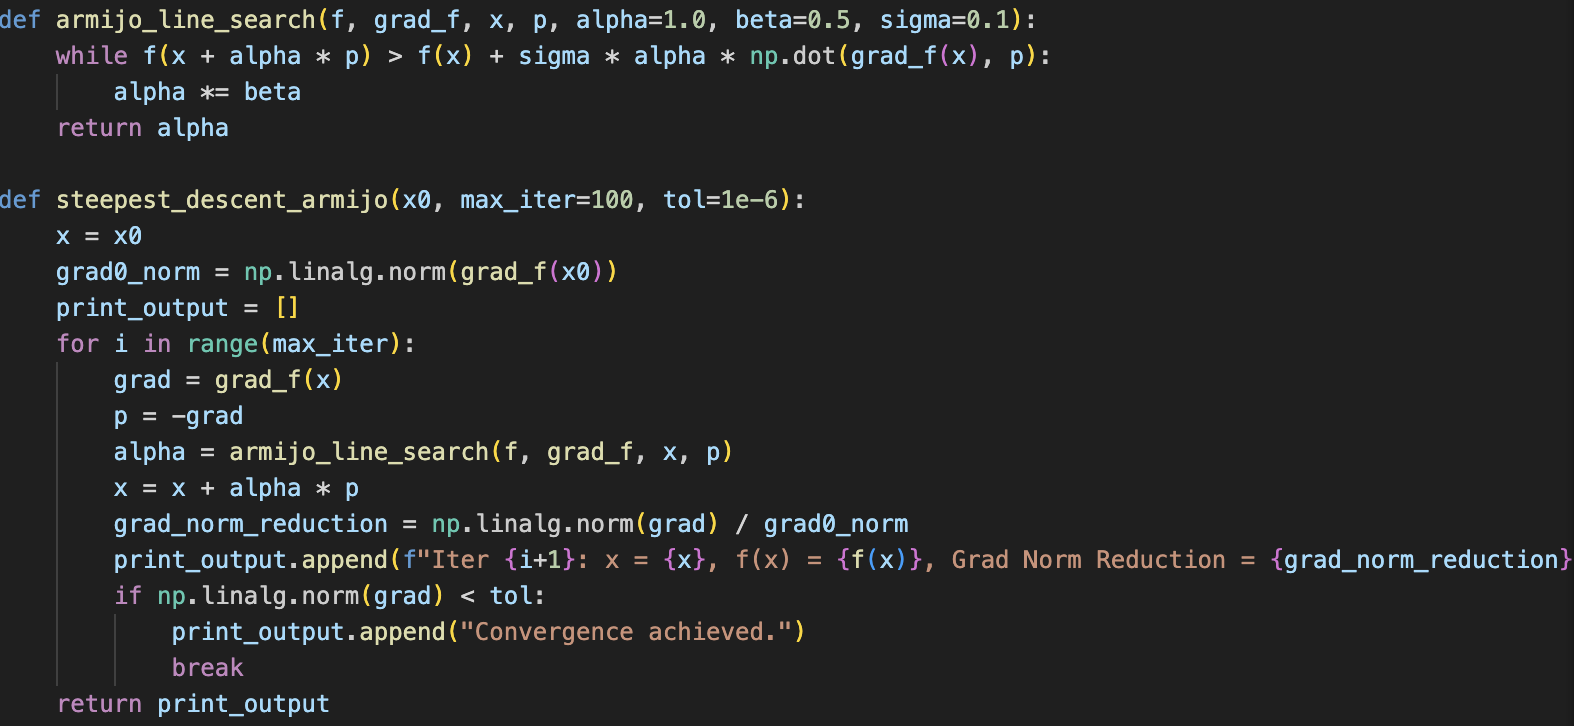
\includegraphics[width=\textwidth]{1a.png} 
    \end{figure}

  
\item At every iteration print out the iteration, the current point
  $x_k$, the value of the objective function $f(x_k)$, the reduction
  in the norm of the gradient $ \|\nabla f(x_k)\|_2/ \|\nabla
  f(x_0)\|_2$, and the step size $\alpha$.

    \begin{figure}[H]
    \centering
    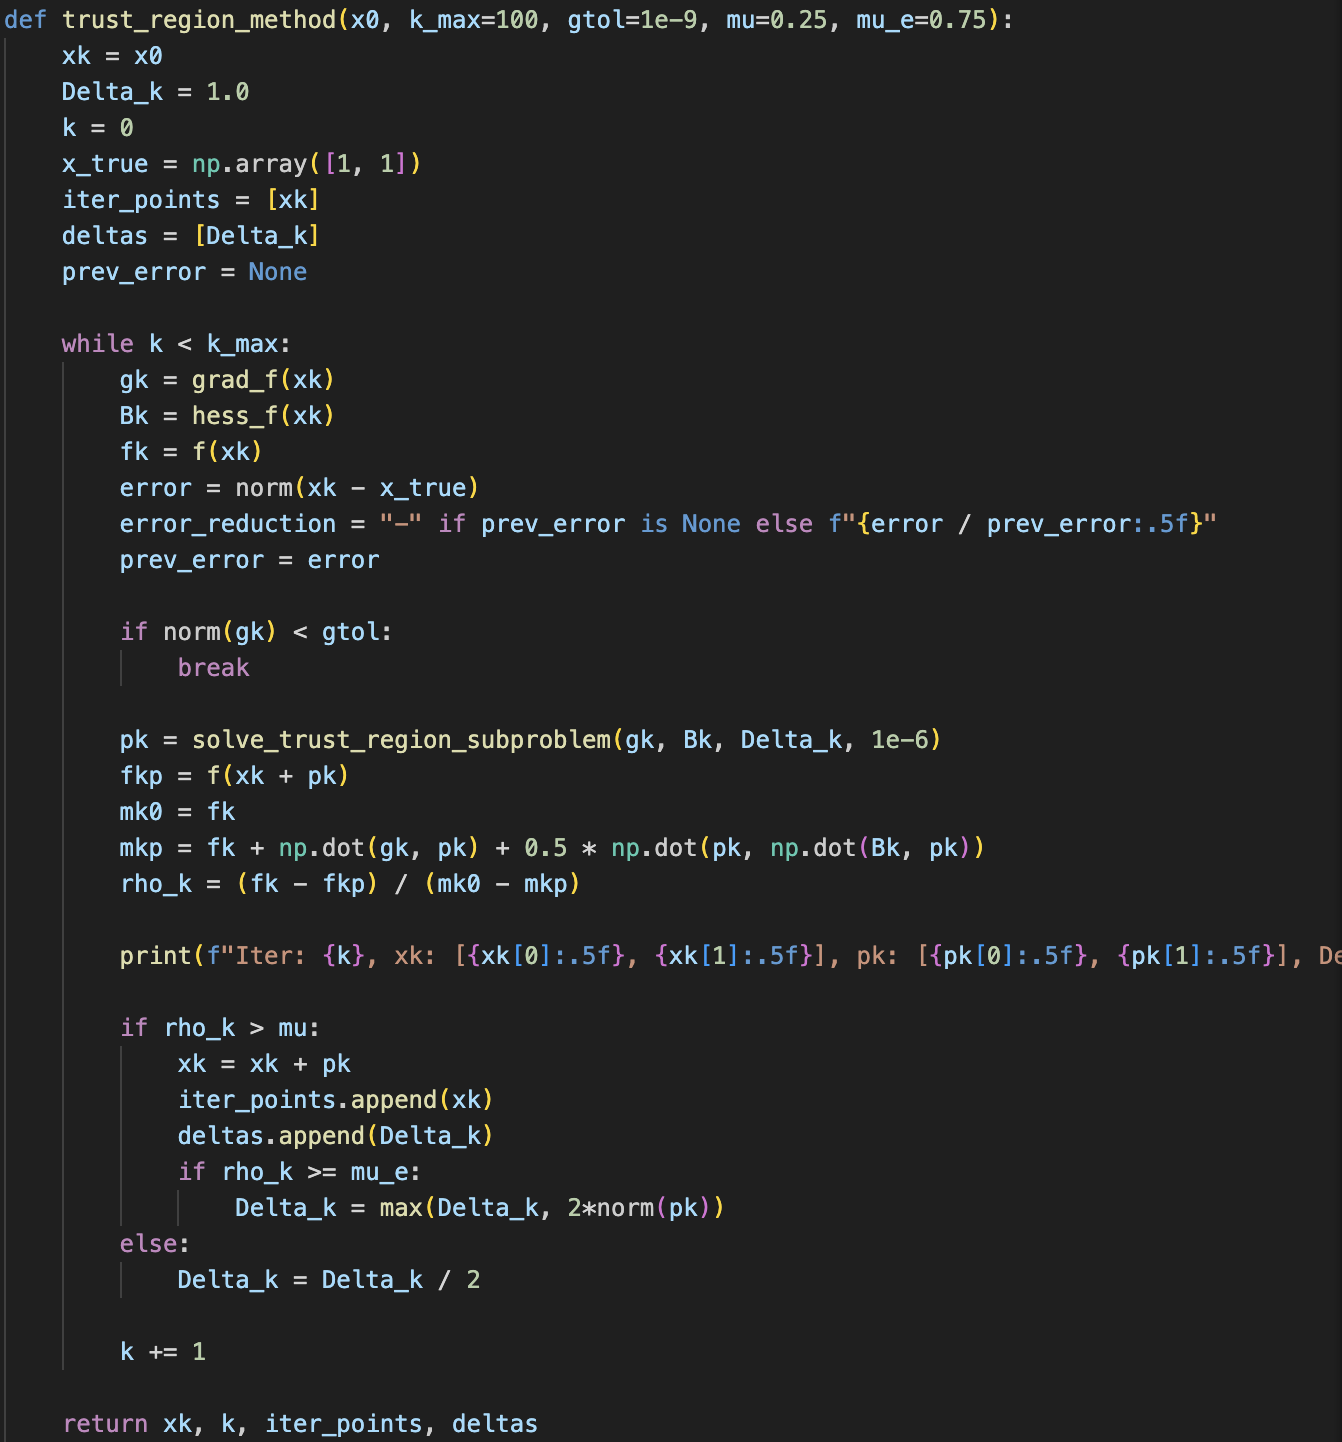
\includegraphics[width=\textwidth]{1b.png} 
    \end{figure}

  
\item Discuss your results.

\textcolor{red}{
Over 50 iterations, the steepest descent algorithm with Armijo line search consistently reduced the objective function \( f(x,y) \), which indicates a steady approach towards a minimum. Starting from \( x_1 = [0.0211, -0.4956] \) with an initial function value of -0.998548, the descent begins close to the function's peak. The trajectory of \( x_k \) values heading towards zero and the marginal decrease in \( y \) values signifies the algorithm's path through the domain, with \( f(x_k) \) lessening at diminishing rates meaning we are approaching into the function's flatter regions. The gradient norm reduction ratio, which initiates at 1.0 and subsequently declines, yet remains above zero, signals an effective yet incomplete convergence. The step size \( \alpha \) is maintained at 1.0 across all iterations. This is not expected since it should be a dynamic adjustment associated with the Armijo line search. This might suggest an aspect of the function's landscape that allows for larger consistent steps or points to a potential need for refinement in the line search criteria to ensure optimality in diverse landscapes.
}




\item Implement Newton's method with Armijo line search and
  backtracking (as discussed in class).  


    \begin{figure}[H]
    \centering
    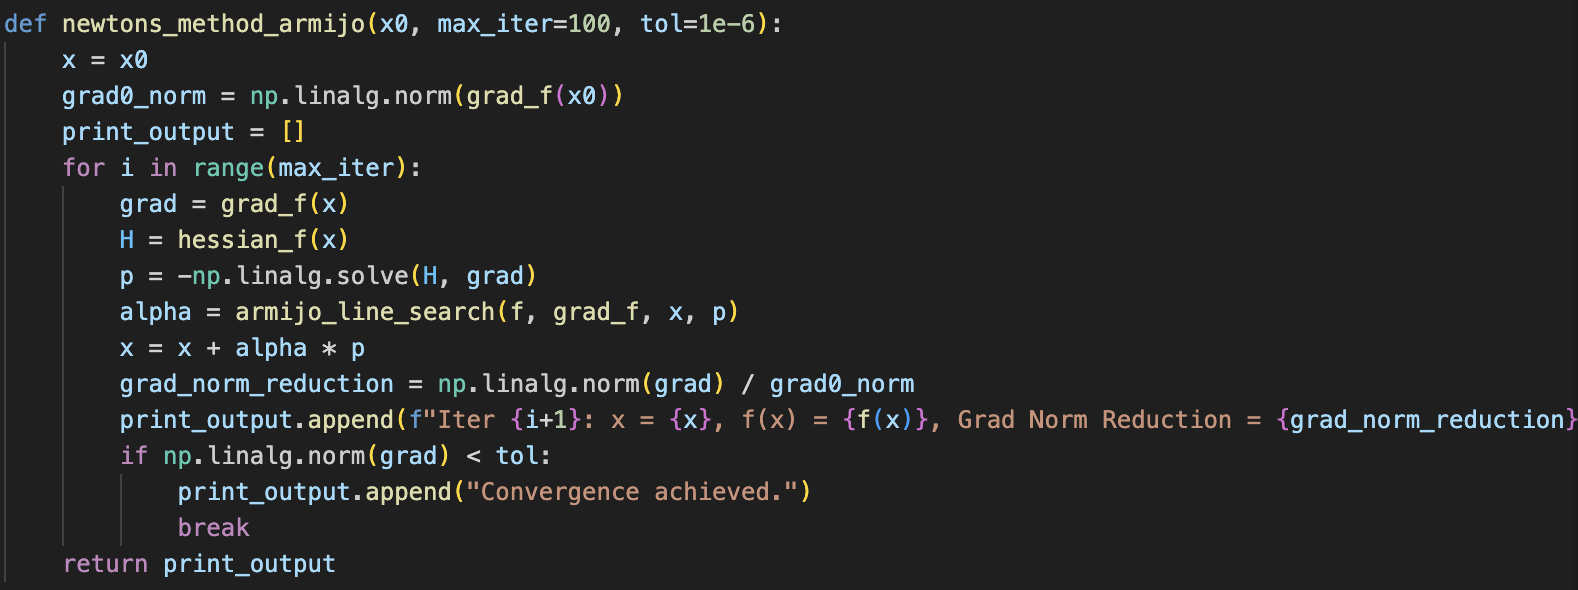
\includegraphics[width=\textwidth]{1d.png} 
    \end{figure}

  
\item Compare the results obtained with steepest descent and Newton's
  method.
  \een


    \begin{figure}[H]
    \centering
    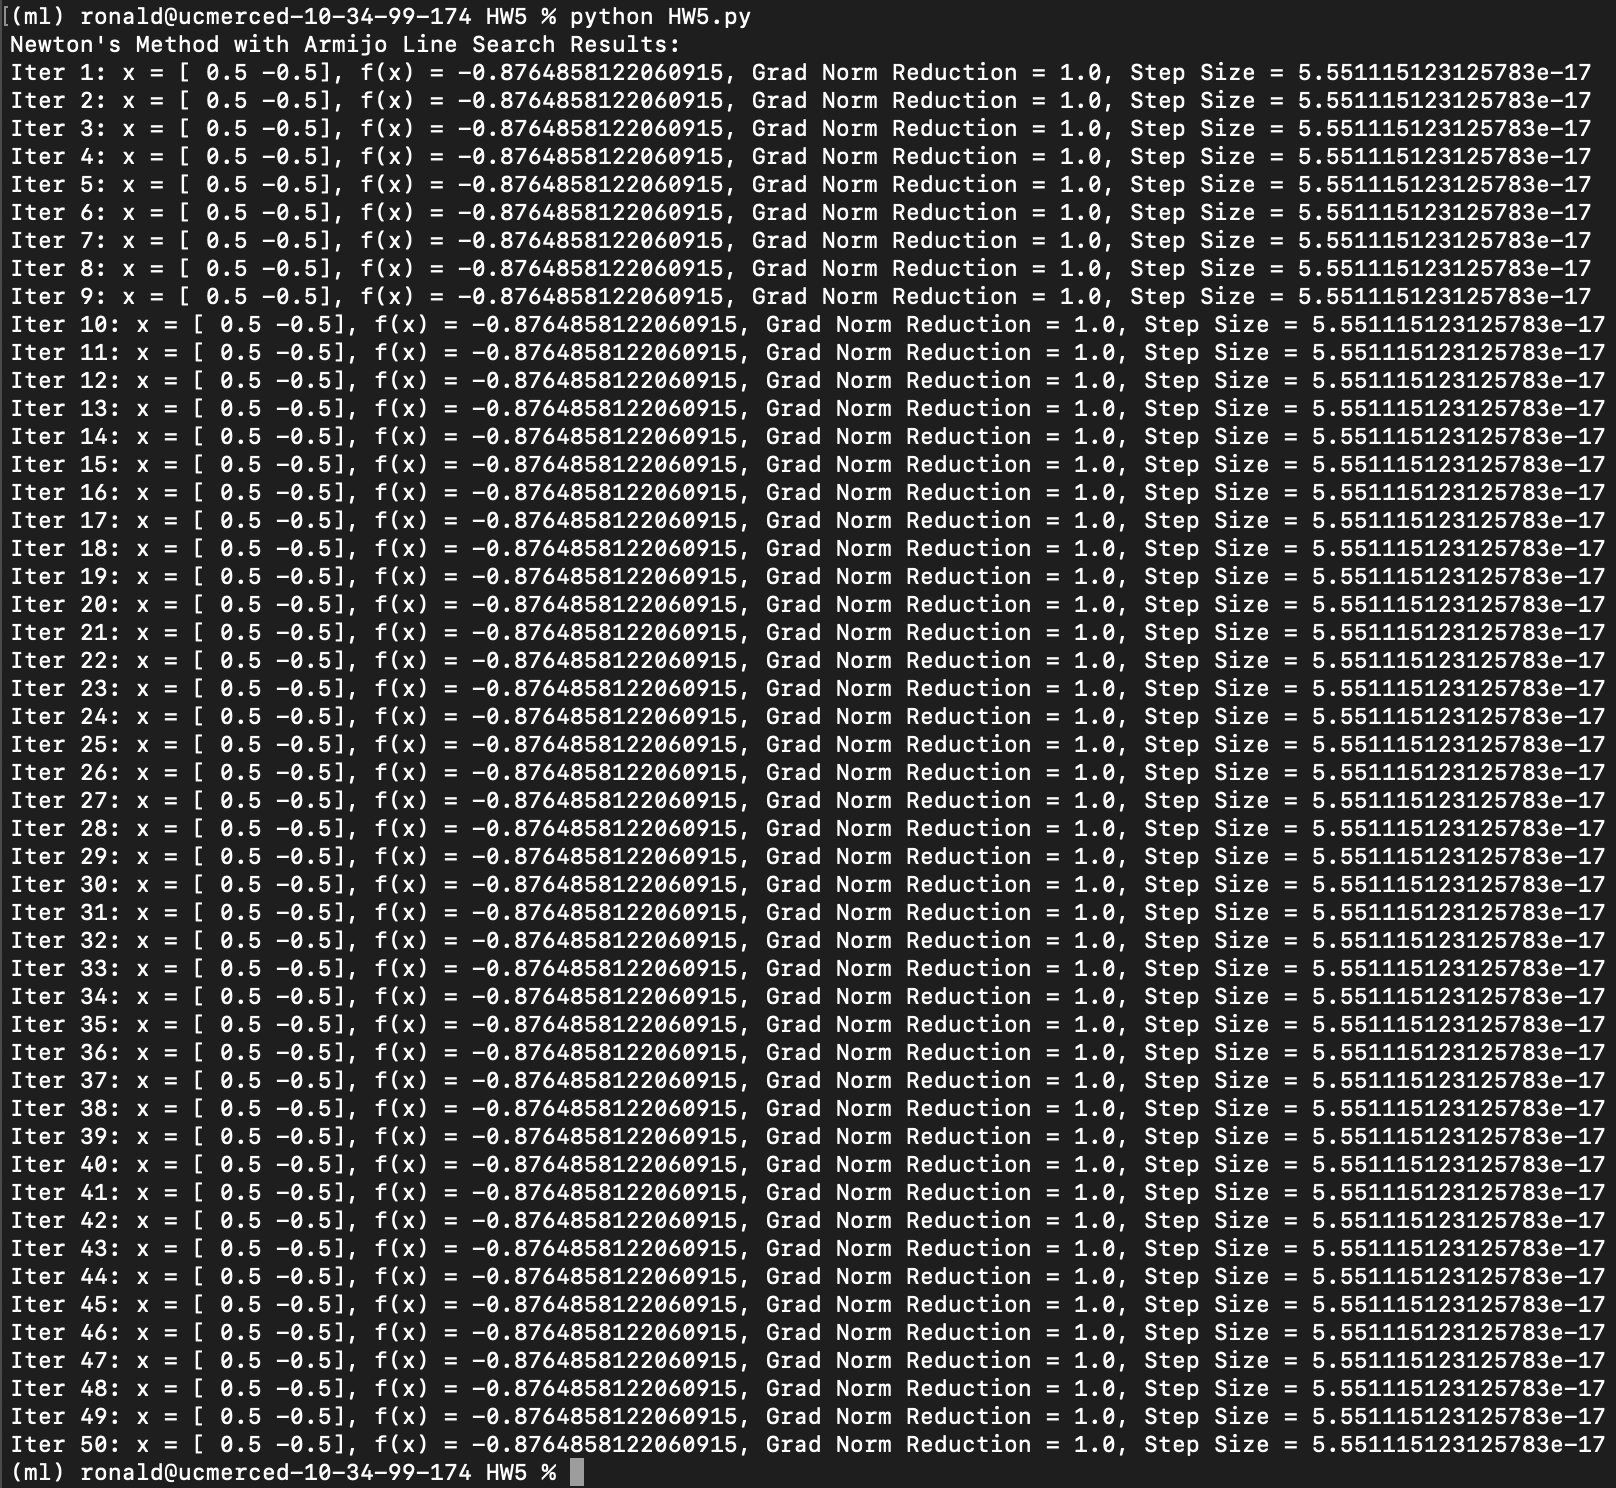
\includegraphics[width=\textwidth]{1e.png} 
    \end{figure}


\textcolor{red}{
Comparing the output of Newton's Method with the Armijo Line Search to those of the Steepest Descent method reveals differences in convergence patterns and efficiency. Newton's Method demonstrates a quick convergence with the function value stabilizing at -0.87648 from the first iteration. The current point \(x = [0.5, -0.5]\) remains unchanged across all iterations, indicating an immediate identification of the optimal point with a minimal step size of \(5.55e^{-17}\). This contrasts with the Steepest Descent method where gradual decreases in the objective function are observed. The constant step size in Newton's Method highlights its efficiency and precision in quickly locating the minimum without the need for iterative adjustments in the direction and magnitude of steps.
}







\item ({\bf 5 points}) {\bf \textcolor{red}{Tentative} Project Plan}:
  \begin{enumerate}
  \item Update your project description, based on latest discussions.

\begin{enumerate}
    \item[\textcolor{red}{Description:}] 
    \textcolor{red}{The project leverages Weighted Least Squares optimization and deep learning for edge-aware image smoothing, aiming to enhance image processing by preserving edges while smoothing backgrounds.}
\end{enumerate}

  \item Write an outline for your project with a timeline.

\begin{enumerate}
    \item[\textcolor{red}{1. Preliminary Study}]
    \textcolor{red}{Conduct literature review and define project scope.}
    
    \item[\textcolor{red}{2. Development}]
    \textcolor{red}{Implement WLS optimization and design the deep learning model.}
    
    \item[\textcolor{red}{3. Evaluation}]
    \textcolor{red}{Assess the methods with metrics.}
    
    \item[\textcolor{red}{4. Documentation}]
    \textcolor{red}{Finalize documentation and outline potential improvements.}
\end{enumerate}

  \end{enumerate}

\end{enumerate}
\end{document}
